% =====================================================================
%  main.tex — HyperPod technical report (compile this file)
%  Build: tectonic main.tex
%
%  Every number in this report comes from a committed log in the
%  repository under test/, or from a command transcript recorded during
%  the run it describes. Nothing is estimated or projected.
% =====================================================================
\documentclass[11pt]{article}
% =====================================================================
%  preamble.tex — shared setup for the HyperPod technical report.
%  Plot conventions follow the common arXiv/NeurIPS single-column look:
%  boxed axes, light grids, small fonts, one solid series with filled
%  markers against one dashed series with open markers.
% =====================================================================
\usepackage[T1]{fontenc}
\usepackage[utf8]{inputenc}
\usepackage[a4paper,margin=1in]{geometry}
\usepackage{amsmath,amssymb}
\usepackage{booktabs}
\usepackage{tabularx}
\usepackage{array}
\usepackage{enumitem}
\usepackage{xcolor}
\usepackage{graphicx}
\usepackage{caption}
\usepackage{tikz}
\usepackage{pgfplots}
\usepackage{listings}
\usepackage{microtype}
\usepackage{fancyhdr}
\usepackage{textcomp}
\usepackage{siunitx}
\sisetup{detect-all,group-separator={,},group-minimum-digits=4}
\usepackage{newunicodechar}
\usepackage[hidelinks]{hyperref}

\pgfplotsset{compat=1.18}
\usepgfplotslibrary{groupplots}
\usetikzlibrary{arrows.meta,positioning,shapes.geometric,calc,fit,backgrounds}

\extrafloats{120}

% ---- Unicode safety -------------------------------------------------
\newunicodechar{→}{\ensuremath{\rightarrow}}
\newunicodechar{≈}{\ensuremath{\approx}}
\newunicodechar{≤}{\ensuremath{\leq}}
\newunicodechar{≥}{\ensuremath{\geq}}
\newunicodechar{×}{\ensuremath{\times}}
\newunicodechar{·}{\ensuremath{\cdot}}
\newunicodechar{–}{--}
\newunicodechar{—}{---}
\newunicodechar{°}{\ensuremath{^\circ}}

% ---- Page furniture -------------------------------------------------
\pagestyle{fancy}
\fancyhf{}
\fancyhead[L]{\small HyperPod — Measured Report}
\fancyhead[R]{\small\thepage}
\renewcommand{\headrulewidth}{0.3pt}

\captionsetup{font=small,labelfont=bf,justification=justified,singlelinecheck=false}

% ---- Column types ---------------------------------------------------
\newcolumntype{Y}{>{\raggedright\arraybackslash}X}
\newcolumntype{R}[1]{>{\raggedleft\arraybackslash}p{#1}}

\newcommand{\code}[1]{\texttt{\small #1}}

% ---- Plot palette ---------------------------------------------------
% One saturated blue and one crimson, as in the reference layout.
\definecolor{serA}{RGB}{31,110,189}   % blue   — solid, filled markers
\definecolor{serB}{RGB}{199,43,104}   % crimson— dashed, open markers
\definecolor{serC}{RGB}{90,100,110}   % slate  — dotted, square markers
\definecolor{panelA}{RGB}{247,250,254}
\definecolor{panelB}{RGB}{254,248,250}

% Shared axis style for every data panel in this report.
\pgfplotsset{
  hpaxis/.style={
    axis lines=box,
    line width=0.35pt,
    grid=both,
    grid style={gray!16,very thin},
    tick align=outside,
    tick style={gray!50,thin},
    tick label style={font=\tiny},
    label style={font=\tiny},
    title style={font=\scriptsize,yshift=1pt},
    legend style={font=\tiny,draw=gray!45,fill=white,fill opacity=0.9,
                  text opacity=1,inner sep=1.6pt,row sep=-1pt},
    legend cell align=left,
    max space between ticks=28,
  },
  solidA/.style={color=serA,mark=*,mark size=1.5pt,line width=0.9pt,
                 mark options={fill=serA,draw=serA}},
  dashedB/.style={color=serB,mark=o,mark size=1.6pt,line width=0.9pt,dashed,
                  mark options={fill=white,draw=serB,solid}},
  dottedC/.style={color=serC,mark=square*,mark size=1.3pt,line width=0.9pt,
                  densely dotted,mark options={fill=serC,draw=serC,solid}},
}


\title{\vspace{-2em}\textbf{HyperPod}\\[0.35em]
\large Measured Placement and Failure Recovery for Meta Llama Models\\
on a Pool of Consumer Laptops\\[0.45em]
\normalsize Technical Report}
\author{\normalsize Dharshaneshwaran\\
\normalsize\textit{Meta Global AI Developer Hackathon --- Indie Developer Track}}
\date{\normalsize 31 October 2026}

\begin{document}
\maketitle
\thispagestyle{fancy}

\begin{abstract}
\noindent
A student or independent developer may own several modest laptops and still have
no single GPU large enough for the local model they want to run. \texttt{llama.cpp}
can already expose a remote accelerator over its RPC backend, so the memory of
several machines can be combined. That backend is documented upstream as a
proof of concept: when one RPC peer disappears, the process that was using it
aborts. Consumer laptops disappear often, which makes the combined pool
difficult to depend on.

This report documents HyperPod, a control plane around \texttt{llama.cpp} that
discovers laptops on a local network, records the hardware each one actually
reports, derives tensor weights from measured free video memory, supervises the
model process, and rebuilds the pipeline when a worker stops answering. It
reports what we measured on three physical machines: a Linux laptop with an
RTX~3050 acting as controller, a Windows laptop with an RTX~4050, and an M4
MacBook~Air running Metal, all on one Wi-Fi network.

Three results are quantified. First, a Llama~3.2~3B model was loaded across all
three machines, and the per-device byte counts reported by \texttt{llama.cpp}
are given. Second, the Mac accelerator was stopped during a request: the
underlying process aborted, HyperPod excluded that endpoint, rebuilt across the
two surviving laptops in \SI{33}{\second}, and the same HTTP request returned.
Under identical conditions, unmodified \texttt{llama.cpp} failed the request and
did not restart. Third, splitting over Wi-Fi was substantially slower than the
single local GPU, at a median of \SI{11.8}{\second} against
\SI{1.54}{\second} per request. HyperPod is therefore a capacity and recovery
mechanism, not an accelerator, and this report states that plainly.
\end{abstract}

\tableofcontents
\clearpage

\section{Introduction}

The hardware a student actually owns is rarely the hardware the tooling assumes.
Over a few years a person may accumulate two or three laptops, each adequate on
its own terms, none of them carrying a large GPU. The machines used throughout
this report are a case in point: a Linux laptop with an RTX~3050 exposing
\SI{4096}{MiB} of video memory, a Windows laptop with an RTX~4050 exposing
\SI{6141}{MiB}, and an M4 MacBook~Air with \SI{16384}{MiB} of unified memory.
Individually, none of them holds a 4.9~GB quantised model in GPU memory.
Together they hold more than enough.

\texttt{llama.cpp} already provides the mechanism for combining them. Its RPC
backend exposes a remote accelerator over TCP, and the main process can offload
model layers to it. The upstream documentation is explicit that this backend is
a proof of concept and that it should not be exposed to untrusted networks. It
is equally explicit in behaviour: if an RPC peer stops responding, the process
using it aborts. We reproduced this directly, and the error text is quoted in
Section~\ref{sec:background}.

That behaviour is the obstacle. A laptop is not a server. Its lid gets closed,
its Wi-Fi roams, its owner stops a terminal. Each of those events ends the
inference process outright, and the model must be loaded again from the
beginning. On the network used here, reloading a 3B model across two machines
took between \SI{33}{\second} and \SI{240}{\second} depending on cache state,
so an unhandled failure is not a brief interruption.

\subsection{What this report covers}

HyperPod is the control plane we built around \texttt{llama.cpp} to make that
pool usable. It does not implement attention kernels, quantisation, or device
offload; \texttt{llama.cpp} performs all of that. HyperPod is responsible for
five things:

\begin{enumerate}[leftmargin=1.4em,itemsep=2pt]
  \item finding worker laptops on the local network without manual addresses;
  \item recording what each laptop reports about its own hardware, and marking
        anything it cannot report as unavailable rather than guessing;
  \item deriving tensor weights from measured free video memory;
  \item reading back the placement \texttt{llama.cpp} actually chose, rather
        than assuming the requested split was honoured;
  \item detecting that the model process has died, excluding the endpoint
        responsible, rebuilding on what remains, and retrying the request that
        was interrupted.
\end{enumerate}

Section~\ref{sec:design} describes the design, including the one scheduling
decision that required a measurement to settle. Section~\ref{sec:results}
reports results from the three machines above: the placement
\texttt{llama.cpp} produced, five-run latency and throughput figures against
two baselines, and two physical failure experiments in which an accelerator was
stopped by hand during a live request.

\subsection{What this report does not claim}

Capability-aware placement across heterogeneous devices is not new, and neither
is failure recovery in distributed serving. Both exist in datacentre systems and
in prior work on consumer-hardware inference, discussed in
Section~\ref{sec:related}. The contribution here is narrower: a working,
measured implementation on three mismatched laptops across CUDA and Metal, with
every claim backed by a committed log, and with the costs reported rather than
omitted.

Three specific costs are reported in full. Splitting over Wi-Fi was roughly six
times slower per output token than the single local GPU. Recovery restarts the
model process and re-runs the request; it does not resume the KV cache or
continue from the token where the failure occurred. And the 8B configuration
demonstrates pooled capacity only: because that model does not fit in the
controller's GPU memory alone, the two-machine arrangement cannot survive the
loss of the remote worker. Each of these is stated again in
Section~\ref{sec:limitations} so that no reader has to infer them.

\section{Background: the failure we had to handle}
\label{sec:background}

\subsection{How the RPC backend distributes a model}

Built with \code{-DGGML\_RPC=ON}, \texttt{llama.cpp} provides
\code{ggml-rpc-server}, which advertises the accelerators of the machine it runs
on. A client passes \code{--rpc host:port} and those remote devices join the
local ones as offload targets. Model layers are then distributed across the
combined set, and \code{--tensor-split} can override the default proportions.

Two properties of this mechanism shaped our design.

First, the device order used by \code{--tensor-split} is not the order printed
by \code{--list-devices}. We established the real order by measurement rather
than by reading documentation, loading the same 3B model twice with opposite
weights:

\begin{center}\small
\begin{tabular}{@{}lrr@{}}
\toprule
\code{--tensor-split} & ROG CUDA0 & TUF RPC0 \\
\midrule
\code{1,4} & \SI{1573}{MiB} & \SI{345}{MiB} \\
\code{4,1} & \SI{552}{MiB}  & \SI{1366}{MiB} \\
\bottomrule
\end{tabular}
\end{center}

Weighting the first position moved memory onto the local GPU, so RPC devices are
listed first and the local device last. Our initial implementation had this
backwards, which placed most of the model on the controller while the logs
claimed it was distributed. Reading the placement back from
\texttt{llama.cpp}, rather than trusting the request, is what exposed the error.

Second, the RPC server accepts one client at a time. While a model is resident,
the device cannot be queried by a second process. We confirmed this when a
device probe aborted against an endpoint already held by the running model. This
rules out querying remote devices for live memory figures during serving, and it
is why worker-reported telemetry is the only usable source.

\subsection{What happens when a worker disappears}

The behaviour on peer loss is unambiguous. With a 3B model split across the
Linux and Windows laptops, we began a request and then stopped the remote
\code{ggml-rpc-server} by hand. \texttt{llama.cpp} emitted:

\begin{quote}\small\ttfamily
Remote RPC server crashed or returned malformed response
\end{quote}

\noindent
and the process aborted. Measured from the client side: \code{curl} exited 52
with HTTP status 000 after \SI{34.06}{\second}, no response body was produced,
the process was gone five seconds later, the health endpoint was unreachable,
and nothing restarted. The model had to be loaded again from scratch.

This is reasonable behaviour for a proof-of-concept backend. A lost peer means
part of the computation graph is unreachable mid-forward-pass, and aborting is
safer than continuing with an incomplete model. The consequence, though, is that
the reliability of the whole pool equals the reliability of its least stable
member. For laptops on Wi-Fi, that is low.

\subsection{The resulting requirement}

Recovery cannot be implemented inside the forward pass without modifying
\texttt{llama.cpp} itself, which we chose not to do: it would fork a fast-moving
upstream project and make the result harder to reproduce. The alternative is to
treat the model process as replaceable and to supervise it from outside. That
places three obligations on the supervisor:

\begin{itemize}[leftmargin=1.4em,itemsep=2pt]
  \item \textbf{Distinguish failure modes.} An ordinary bad request must not
        trigger a rebuild, and a dead worker must not be mistaken for one. We
        settled on process exit as the signal, for reasons given in
        Section~\ref{sec:design}.
  \item \textbf{Verify endpoints independently of agent health.} A worker's
        heartbeat proves its agent is running, not that its accelerator is
        reachable. The experiment in Section~\ref{sec:recovery} was designed
        specifically to separate these two states.
  \item \textbf{Preserve the interrupted request.} A user who submitted a
        prompt before the failure should not have to resubmit it.
\end{itemize}

\section{Design}
\label{sec:design}

\subsection{Components}

HyperPod has three parts: a Go controller on the machine the user sits at, a
Rust agent on every laptop that contributes compute, and a React dashboard.
Figure~\ref{fig:arch} shows how they relate to the \texttt{llama.cpp} processes
that perform the actual inference.

\begin{figure}[htbp]
\centering
\begin{tikzpicture}[font=\scriptsize,
  box/.style={draw=gray!55,rounded corners=2pt,align=center,inner sep=4pt,line width=0.4pt},
  mach/.style={box,text width=3.05cm,align=center},
  rstep/.style={box,text width=2.75cm,align=center},
  lnk/.style={-{Stealth[length=4pt]},gray!65,line width=0.5pt}]

% ---- row 1: dashboard and control plane ----
\node[box,text width=2.1cm] (ui) at (-4.85,3.25)
  {\textbf{Dashboard}\\[1pt]{\tiny telemetry}\\[-1pt]{\tiny placement}};
\node[box,fill=serA!10,draw=serA!65,text width=7.4cm] (cp) at (1.55,3.25)
  {\textbf{Go controller}\\[2.5pt]
   {\tiny registry \ \textbar\ \ measured-VRAM scheduler \ \textbar\ \ supervisor \ \textbar\ \ retry}};
\draw[lnk] (ui) -- node[above,font=\tiny,inner sep=2pt]{HTTP} (cp);

% ---- row 2: machines ----
\node[mach,fill=serA!7,draw=serA!50]        (rog) at (-3.35,1.05)
  {\textbf{ROG} · Linux\\[1pt]{\tiny controller + \code{llama-server}}\\[-1pt]{\tiny RTX 3050 · local CUDA}};
\node[mach,fill=green!6,draw=green!40!black!45] (tuf) at (0.45,1.05)
  {\textbf{TUF} · Windows\\[1pt]{\tiny agent + \code{ggml-rpc-server}}\\[-1pt]{\tiny RTX 4050 · remote CUDA}};
\node[mach,fill=orange!8,draw=orange!60!black!40] (mac) at (4.25,1.05)
  {\textbf{M4 Mac} · macOS\\[1pt]{\tiny agent + \code{ggml-rpc-server}}\\[-1pt]{\tiny remote Metal}};

\draw[lnk] (cp.south -| rog.north) -- node[left,font=\tiny,inner sep=1.5pt]{local} (rog.north);
\draw[lnk] (cp.south -| tuf.north) -- node[right,font=\tiny,inner sep=1.5pt]{RPC / Wi-Fi} (tuf.north);
\draw[lnk] (cp.south -| mac.north) -- node[right,font=\tiny,inner sep=1.5pt]{RPC / Wi-Fi} (mac.north);

% discovery / heartbeat path back to the registry
\draw[lnk,serB,dashed] (rog.south) -- ++(0,-0.45) -- (6.35,-0.45) -- (6.35,3.25) -- (cp.east);
\node[font=\tiny,text=serB,anchor=south] at (1.0,-0.42) {discovery · heartbeat · telemetry};

% ---- row 3: recovery sequence ----
\node[rstep,fill=serB!7,draw=serB!50]            (f1) at (-3.35,-1.75)
  {accelerator stops\\[1pt]{\tiny \code{llama-server} aborts}};
\node[rstep,fill=serA!8,draw=serA!50]            (f2) at (0.45,-1.75)
  {endpoint excluded\\[1pt]{\tiny rebuild on survivors}};
\node[rstep,fill=green!7,draw=green!40!black!45] (f3) at (4.25,-1.75)
  {same request retried\\[1pt]{\tiny response returned}};
\draw[lnk,serB,dashed] (f1) -- (f2);
\draw[lnk,serA] (f2) -- (f3);
\end{tikzpicture}
\caption{HyperPod components and the recovery path. \texttt{llama.cpp} performs
all inference; the Go controller decides placement, observes it, and replaces
the model process when a worker stops answering. The bottom row is the sequence
measured in Section~\ref{sec:recovery}.}
\label{fig:arch}
\end{figure}

\subsection{Telemetry that refuses to guess}

Each agent samples its own hardware every five seconds and reports the snapshot
with registration, with every heartbeat, and in its discovery broadcast. The
schema is versioned, and the controller rejects a version it does not
understand.

The design rule that mattered most is that every value which can be unavailable
is nullable, and an unavailable value is transmitted as \code{null} rather than
as zero or as a plausible substitute. Three cases from our own hardware show why:

\begin{itemize}[leftmargin=1.4em,itemsep=2pt]
  \item The Windows RTX~4050 reports no GPU power limit; \code{nvidia-smi}
        returns \code{[N/A]}. That field stays \code{null}.
  \item Apple Silicon has one unified memory pool, so there is no separate
        free-video-memory quantity. Reporting system RAM in that field would
        imply a dedicated figure that does not exist, so it stays \code{null}.
  \item macOS exposes no direct equivalent of \code{MemAvailable}. We derive
        available memory from \code{vm\_stat} page classes and name that source
        explicitly, so a reader can judge the estimate.
\end{itemize}

Sources are carried in the payload (\code{nvidia-smi}, \code{windows-cim},
\code{macos-sysctl+vm\_stat}, and so on) and shown in the dashboard, so no
number in the interface is anonymous.

\subsection{Deriving the split from measurement}

When every selected device reports free video memory, the controller computes

\[
w_i \;=\; \mathrm{free\_vram}_i \;-\; R, \qquad R = \SI{512}{MiB},
\]

where $R$ is a fixed reserve held back on each device for runtime buffers, and
the resulting $w_i$ are passed to \code{--tensor-split} in RPC-first order.
Endpoints are sorted before the weights are built, so the same measurements
always produce the same argument string. $R$ is a policy choice, not a
measurement, and it is labelled as such in the interface.

If any required value is missing --- as with the Mac --- the controller supplies
no weights at all and records the strategy as
\code{llama.cpp-auto (remote free VRAM unavailable)}. \texttt{llama.cpp} then
probes the devices itself. We preferred this to deriving a weight from a GPU
name or from total memory, because a wrong weight produces a silently
unbalanced model rather than a visible gap.

\subsection{Choosing the failure signal}

Detecting worker loss was the hardest design decision, and our first two
attempts were wrong.

Port probing was too eager: a TCP connection can succeed against a socket whose
server is no longer serving, and it can fail transiently on a busy Wi-Fi link.
Health polling was no better, because a loaded model can be slow to answer
while remaining healthy.

The signal we settled on is the exit of the supervised \code{llama-server}
process. When an RPC peer is lost, \texttt{llama.cpp} aborts, so the process
exit is both reliable and specific. Two refinements were needed:

\begin{itemize}[leftmargin=1.4em,itemsep=2pt]
  \item \textbf{Loading is not failure.} A model still loading answers health
        checks with 503. An early version treated that as death and killed its
        own load. Readiness is now watched by a separate observer with no
        timeout, and a request that arrives during loading waits and is then
        told the model is still loading.
  \item \textbf{The abort and the client error race.} The HTTP request fails
        milliseconds before the process exit is observed. A failed request
        therefore waits up to five seconds to see whether the process exits
        before it is classified as an ordinary error.
\end{itemize}

On rebuild, every candidate endpoint is probed directly. A worker whose
heartbeat is healthy but whose accelerator is unreachable is excluded, which is
exactly the condition tested in Section~\ref{sec:recovery}.

\section{Implementation}

The repository contains roughly 3{,}570 lines of our own code across three
languages, excluding the vendored \texttt{llama.cpp} checkout and generated
dependency files.

\subsection{Go controller}

The controller owns cluster state and the model process. It exposes
\code{POST /register}, \code{POST /heartbeat}, \code{GET /status},
\code{GET /pipeline} and \code{POST /infer}, and listens for discovery
broadcasts on UDP~50999. A worker is considered healthy if its last heartbeat
arrived within ten seconds.

Two implementation details are worth recording because both were bugs first.

The placement reader parses \texttt{llama.cpp}'s own load output. Running the
model server at log verbosity~4 makes it print one line per device of the form
\code{load\_tensors: <device> model buffer size = <N> MiB}, which the controller
captures into structured per-device figures. This is the only reason we noticed
the reversed tensor-split order described in Section~\ref{sec:background}: the
requested weights and the actual placement disagreed.

The process is started from the directory holding the \texttt{llama.cpp}
binaries. Renaming the project directory broke the build until we fixed this,
because the server resolves its shared libraries relative to its own location
and exited with status~127 before contacting any worker.

\subsection{Rust worker}

One agent binary serves Windows, Linux and macOS. It broadcasts presence,
registers, heartbeats every three seconds, and re-registers automatically if a
heartbeat fails, which is what allows the cluster to reassemble after the
controller restarts.

A single sampler runs every five seconds and its snapshot is shared by all three
message paths. This matters on Windows, where each sample would otherwise spawn
separate PowerShell and \code{nvidia-smi} processes for registration,
heartbeats and discovery.

\begin{table}[htbp]
\centering\small
\caption{Telemetry sources per platform. Every value these tools decline to
report is transmitted as \code{null}.}
\label{tab:sources}
\begin{tabular}{@{}llll@{}}
\toprule
 & \textbf{GPU} & \textbf{Memory} & \textbf{Power} \\
\midrule
Linux (NVIDIA)   & \code{nvidia-smi} & \code{/proc/meminfo} & \code{/sys/class/power\_supply} \\
Windows (NVIDIA) & \code{nvidia-smi} & CIM & CIM + WMI \\
macOS            & \code{system\_profiler} (name only) & \code{sysctl} + \code{vm\_stat} & \code{pmset} \\
\bottomrule
\end{tabular}
\end{table}

On macOS the chipset name is resolved once and cached, because
\code{system\_profiler} is slow and the value never changes, while memory and
power are sampled on every cycle.

\subsection{Dashboard}

The React dashboard polls \code{/status} and \code{/pipeline}. It shows the
topology, per-node measured hardware, the scheduler strategy with the exact
weights it produced, and the placement \texttt{llama.cpp} reported. Fields the
worker could not measure render as \textit{Unavailable}, never as zero.

\subsection{Tests}

Fifteen unit tests cover the parts where a silent error would be most damaging:
seven in Go and eight in Rust. They assert that unavailable values survive as
\code{null} through serialisation, that \code{[N/A]} fields are not coerced to
zero, that real \code{nvidia-smi} and \code{vm\_stat} output parses correctly,
that malformed output is rejected rather than half-read, that identical
measurements always yield identical tensor weights, that a missing measurement
produces the documented fallback instead of an invented weight, and that a
heartbeat carrying no telemetry does not erase the previous snapshot.

Continuous integration was deliberately left out of scope. All checks are run
locally: \code{go test}, \code{go vet}, \code{cargo test}, \code{cargo clippy}
with warnings as errors, and a TypeScript production build with zero lint
warnings.

\section{Experimental setup}
\label{sec:setup}

\subsection{Machines}

All three machines are personally owned consumer laptops on one domestic Wi-Fi
network. Nothing was rented, and no datacentre hardware was involved.

\begin{table}[htbp]
\centering\small
\caption{Hardware. Video memory figures are as reported by the machine itself
through the sources in Table~\ref{tab:sources}.}
\label{tab:hardware}
\begin{tabular}{@{}lllrr@{}}
\toprule
\textbf{Role} & \textbf{Machine} & \textbf{Accelerator} & \textbf{GPU memory} & \textbf{System RAM} \\
\midrule
Controller      & ASUS ROG, Linux   & RTX 3050 Laptop, CUDA & \SI{4096}{MiB} & \SI{15234}{MiB} \\
Remote worker   & ASUS TUF, Windows & RTX 4050 Laptop, CUDA & \SI{6141}{MiB} & \SI{16003}{MiB} \\
Remote worker   & MacBook Air, macOS & Apple M4, Metal      & unified        & \SI{16384}{MiB} \\
\bottomrule
\end{tabular}
\end{table}

The Mac row carries no separate GPU memory figure because Apple Silicon has no
separate pool to report. Its \SI{16384}{MiB} is one unified allocation shared
between CPU and GPU.

\subsection{Software}

Both NVIDIA machines run \texttt{llama.cpp} release \code{b11909}, built with
CUDA and RPC support, at RPC protocol 8.0.1. The Mac runs the official
\code{b11909} macOS arm64 build. Keeping one release across all three machines
removed protocol mismatch as a variable. Every remote
\code{ggml-rpc-server} runs with \code{-c}, which caches received tensors on the
worker's own disk so that only the first load transfers weights over Wi-Fi.

\subsection{Models}

\begin{itemize}[leftmargin=1.4em,itemsep=2pt]
  \item \textbf{Llama 3.2 1B Instruct}, Q4\_K\_M --- local fallback profile.
  \item \textbf{Llama 3.2 3B Instruct}, Q4\_K\_M, \SI{2.0}{GB} --- used for every
        split and recovery experiment. It fits in the controller's GPU alone,
        which is what allows the controller to take over after a worker is lost.
  \item \textbf{Llama 3.1 8B Instruct}, Q4\_K\_M, \SI{4.9}{GB} --- capacity
        experiment. Verified byte-for-byte against the published artefact. It
        does not fit in the controller's \SI{4096}{MiB} GPU alone.
\end{itemize}

No weights are committed to the repository. Context length was 2{,}048 tokens
throughout.

\subsection{Network}

A \SI{5}{GHz} Wi-Fi network. Link conditions were recorded at measurement time
because they are the dominant variable in every distributed figure here. During
the benchmark runs of Section~\ref{sec:perf} the controller reported
\SI{-56}{dBm} with driver-reported rates of \SI{780}{Mbit/s} receive and
\SI{292.5}{Mbit/s} transmit. During the earliest model transfers, several days
before, the same link reported \SI{-66}{dBm} to \SI{-68}{dBm} and
\SI{26}{Mbit/s} to \SI{29}{Mbit/s} transmit. These are physical-layer rates
negotiated by the driver, not achieved application throughput, and the gap
between the two sessions explains why first-load times differ so widely in
Section~\ref{sec:load}.

\subsection{Method}

Performance figures come from five sequential requests against an
already-loaded model, using one fixed prompt asking for a 100-word explanation
of distributed computing, capped at 160 output tokens. Normal sampling was left
enabled, so output lengths vary slightly between runs; we therefore report
medians and full ranges rather than a single best run. End-to-end latency is
\code{curl}'s \code{time\_total}. Decode throughput is taken from
\texttt{llama.cpp}'s own per-request timing line, using the \code{eval time}
figure and excluding \code{prompt eval time}; it is never derived from response
character counts.

Three configurations were measured:

\begin{enumerate}[leftmargin=1.4em,itemsep=2pt]
  \item \textbf{Local baseline} --- \texttt{llama.cpp} on the controller alone,
        no RPC.
  \item \textbf{Native split} --- \texttt{llama.cpp} directly, with the Windows
        RPC endpoint and the same tensor weights HyperPod had computed.
  \item \textbf{HyperPod split} --- the same split reached through the Go
        controller.
\end{enumerate}

Comparing the second and third isolates the control plane, since the inference
path is identical. Failure experiments were performed by stopping a
\code{ggml-rpc-server} process by hand while a request was in flight; no
failures were simulated in software for the results reported here.

\section{Results}
\label{sec:results}

\subsection{Measured telemetry}

Before any model was loaded, the workers reported the figures in
Table~\ref{tab:telemetry}. These are the values the scheduler consumes.

\begin{table}[htbp]
\centering\small
\caption{Worker telemetry as received by the controller. Dashes mark fields the
platform does not expose; these are transmitted as \code{null} and shown in the
dashboard as \textit{Unavailable}.}
\label{tab:telemetry}
\begin{tabular}{@{}lrr@{}}
\toprule
 & \textbf{TUF (Windows)} & \textbf{M4 Mac} \\
\midrule
GPU name           & RTX 4050 Laptop   & Apple M4 \\
GPU memory, free / total & \SI{5843}{} / \SI{6141}{MiB} & --- \\
GPU utilisation    & \SI{0}{\percent}  & --- \\
GPU temperature    & \SI{50}{\celsius} & --- \\
GPU power draw     & \SI{4.09}{W}      & --- \\
GPU power limit    & ---               & --- \\
System RAM, available / total & \SI{4845}{} / \SI{16003}{MiB} & \SI{5938}{} / \SI{16384}{MiB} \\
Battery, AC        & \SI{84}{\percent}, online & \SI{16}{\percent}, online \\
\bottomrule
\end{tabular}
\end{table}

The Windows GPU power limit is blank because \code{nvidia-smi} returned
\code{[N/A]} on that machine. The Mac's GPU rows are blank because macOS
publishes no per-GPU memory, utilisation, temperature or power figure for Apple
Silicon through the interfaces we use. Both cases are reported as unavailable
rather than filled with a substitute.

\subsection{Scheduling and actual placement}

With both NVIDIA devices reporting free memory, the scheduler produced weights
directly from measurement:

\[
\underbrace{5843 - 512}_{\text{TUF RPC}} = 5331,
\qquad
\underbrace{3716 - 512}_{\text{ROG local}} = 3204,
\qquad\Rightarrow\quad
\texttt{--tensor-split 5331,3204}
\]

Figure~\ref{fig:placement} shows the placement \texttt{llama.cpp} subsequently
reported for four configurations. These are read back from its load output, not
inferred from the request.

\begin{figure}[htbp]
\centering
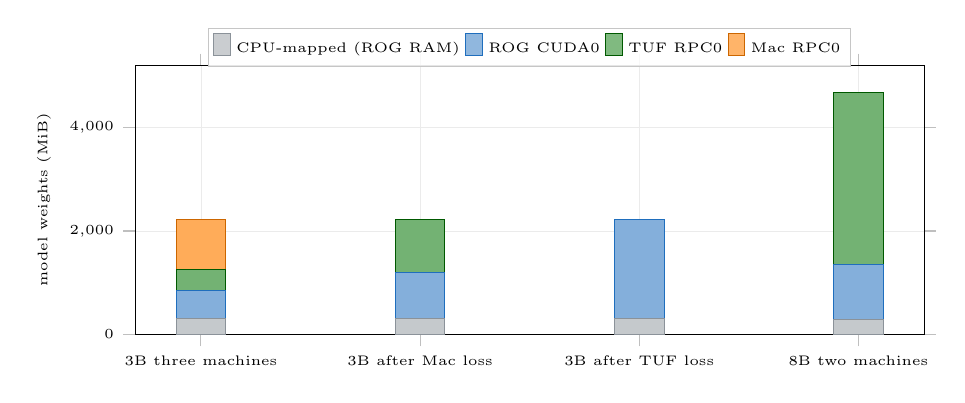
\begin{tikzpicture}[font=\scriptsize]
\begin{axis}[hpaxis,
  width=11.6cm,height=5.0cm,
  ybar stacked, bar width=18pt,
  ymin=0,ymax=5200,
  ylabel={model weights (MiB)},
  symbolic x coords={3B three machines,3B after Mac loss,3B after TUF loss,8B two machines},
  xtick=data,
  x tick label style={font=\tiny,align=center},
  legend style={at={(0.5,1.14)},anchor=north,legend columns=4,draw=gray!45},
  nodes near coords={},
  grid=major,
  ]
% CPU-mapped
\addplot+[fill=serC!35,draw=serC!70,bar shift=0pt]
  coordinates {(3B three machines,308) (3B after Mac loss,308) (3B after TUF loss,308) (8B two machines,282)};
% ROG local CUDA
\addplot+[fill=serA!55,draw=serA,bar shift=0pt]
  coordinates {(3B three machines,552) (3B after Mac loss,896) (3B after TUF loss,1918) (8B two machines,1073)};
% TUF RPC
\addplot+[fill=green!45!black!55,draw=green!35!black,bar shift=0pt]
  coordinates {(3B three machines,398) (3B after Mac loss,1022) (3B after TUF loss,0) (8B two machines,3330)};
% Mac RPC
\addplot+[fill=orange!65,draw=orange!80!black,bar shift=0pt]
  coordinates {(3B three machines,968) (3B after Mac loss,0) (3B after TUF loss,0) (8B two machines,0)};
\legend{CPU-mapped (ROG RAM), ROG CUDA0, TUF RPC0, Mac RPC0}
\end{axis}
\end{tikzpicture}
\caption{Per-device model weights reported by \texttt{llama.cpp} after loading,
for four measured configurations. The first two bars are the same request
before and after the Mac accelerator was stopped: its \SI{968}{MiB} is
redistributed onto the two surviving machines. The fourth bar is the 8B
capacity run, where the remote Windows GPU holds \SI{3330}{MiB} of the
\SI{4.9}{GB} model.}
\label{fig:placement}
\end{figure}

Two observations follow from the figure. In the three-machine configuration the
Mac received the largest remote share, \SI{968}{MiB}, even though HyperPod
supplied no weights for it; that allocation was \texttt{llama.cpp}'s own
decision under the documented fallback. And in the 8B run the remote Windows GPU
holds \SI{3330}{MiB} against \SI{1073}{MiB} on the controller. That is
\SI{71}{\percent} of all reported model weights, or \SI{76}{\percent} of the
weights resident on a GPU, and it is what makes that model runnable at all on
this hardware.

\subsection{Latency and throughput}
\label{sec:perf}

Figure~\ref{fig:perf} gives all five runs for each configuration. We plot every
run rather than only the medians, because the run-to-run spread is the most
important feature of the distributed measurements.

\begin{figure}[htbp]
\centering
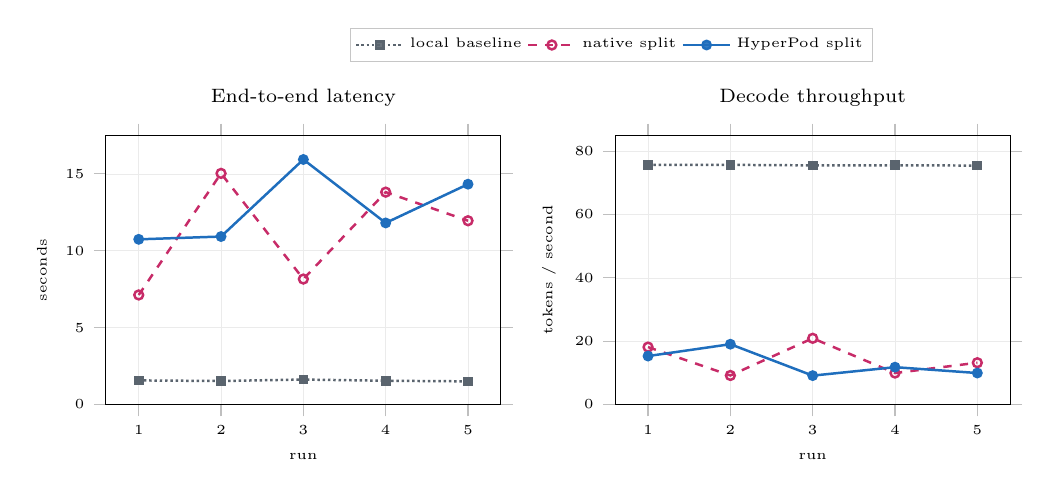
\begin{tikzpicture}[font=\scriptsize]
\begin{groupplot}[group style={group size=2 by 1,horizontal sep=1.45cm},
  hpaxis,width=6.6cm,height=5.0cm,xmin=0.6,xmax=5.4,xtick={1,2,3,4,5},
  xlabel={run},]

\nextgroupplot[title={End-to-end latency},ylabel={seconds},ymin=0,ymax=17.5,
  legend style={at={(1.28,1.40)},anchor=north,legend columns=3,draw=gray!45}]
\addplot+[dottedC] coordinates {(1,1.566)(2,1.527)(3,1.623)(4,1.543)(5,1.505)};
\addlegendentry{local baseline}
\addplot+[dashedB] coordinates {(1,7.122)(2,15.025)(3,8.157)(4,13.807)(5,11.947)};
\addlegendentry{native split}
\addplot+[solidA] coordinates {(1,10.739)(2,10.920)(3,15.930)(4,11.804)(5,14.324)};
\addlegendentry{HyperPod split}

\nextgroupplot[title={Decode throughput},ylabel={tokens / second},ymin=0,ymax=85]
\addplot+[dottedC] coordinates {(1,75.64)(2,75.68)(3,75.51)(4,75.54)(5,75.45)};
\addplot+[dashedB] coordinates {(1,18.13)(2,9.17)(3,20.91)(4,9.94)(5,13.19)};
\addplot+[solidA] coordinates {(1,15.30)(2,19.04)(3,9.12)(4,11.79)(5,9.94)};
\end{groupplot}
\end{tikzpicture}
\caption{Five sequential requests per configuration against a warm model.
The local baseline is tightly clustered, varying by \SI{0.12}{\second} and
\SI{0.23}{tokens/second} across all five runs. Both distributed configurations
vary by several seconds and by more than a factor of two in throughput, which
we attribute to the Wi-Fi link rather than to the control plane.}
\label{fig:perf}
\end{figure}

\begin{table}[htbp]
\centering\small
\caption{Medians and ranges over the five runs of Figure~\ref{fig:perf}.}
\label{tab:perf}
\begin{tabular}{@{}lrrrr@{}}
\toprule
\textbf{Configuration} & \textbf{Median latency} & \textbf{Range} & \textbf{Median decode} & \textbf{Range} \\
\midrule
Local baseline  & \SI{1.543}{\second}  & 1.505--1.623 & \SI{75.54}{} & 75.45--75.68 \\
Native split    & \SI{11.947}{\second} & 7.122--15.025 & \SI{13.19}{} & 9.17--20.91 \\
HyperPod split  & \SI{11.804}{\second} & 10.739--15.930 & \SI{11.79}{} & 9.12--19.04 \\
\bottomrule
\end{tabular}
\end{table}

The local baseline decoded at a median \SI{75.54}{tokens/second} against
\SI{11.79}{} for the HyperPod split: distributing this model over this Wi-Fi
network cost roughly a factor of six in throughput. That is the central cost of
the approach and we do not present it as anything else.

Between the two distributed configurations the median latencies differ by
\SI{0.143}{\second}, which is far smaller than the spread within either
configuration: \SI{5.2}{\second} for the HyperPod split and \SI{7.9}{\second}
for the native split. With five runs we can state that the control plane
introduced no latency penalty large enough to separate from link variance; we
cannot make a stronger claim than that, and a larger sample would be needed to
try.

\subsection{Failure and recovery}
\label{sec:recovery}

Three failure experiments were run, all by stopping a real
\code{ggml-rpc-server} process by hand during a live request.
Figure~\ref{fig:timeline} shows them on a common time axis.

\begin{figure}[htbp]
\centering
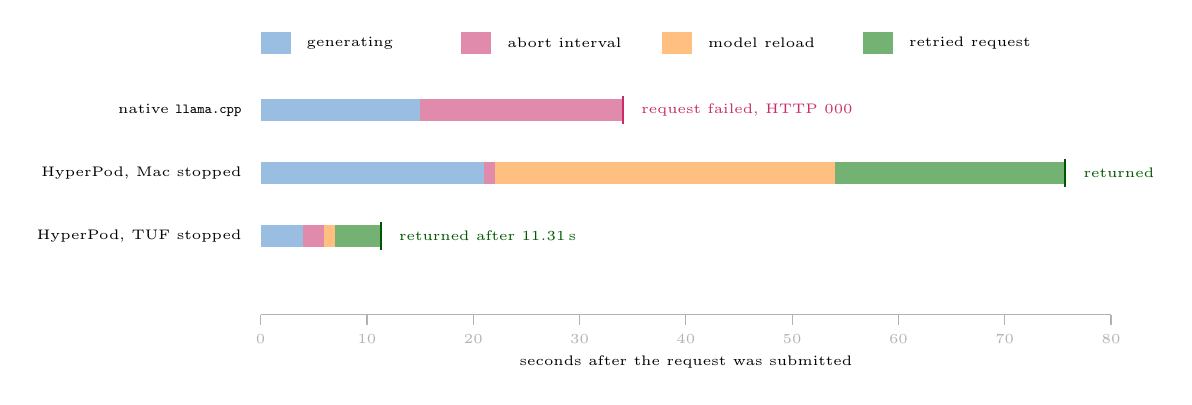
\begin{tikzpicture}[font=\scriptsize,
  lbl/.style={anchor=east,font=\tiny},
  bar/.style={line width=8pt},
  tick/.style={gray!60,line width=0.4pt},
  outlbl/.style={font=\tiny,anchor=west}]

\def\sx{0.135}   % seconds -> cm

% legend
\begin{scope}[shift={(0,2.95)}]
  \foreach \i/\c/\t in {0/serA!45/generating, 1/serB!55/abort interval,
                        2/orange!50/model reload, 3/green!45!black!55/retried request}{
    \draw[bar,\c] (\i*2.55,0) -- (\i*2.55+0.38,0);
    \node[font=\tiny,anchor=west] at (\i*2.55+0.46,0) {\t};
  }
\end{scope}

% axis
\draw[tick] (0,-0.5) -- (80*\sx,-0.5);
\foreach \t in {0,10,20,30,40,50,60,70,80}{
  \draw[tick] (\t*\sx,-0.5) -- (\t*\sx,-0.63) node[below,font=\tiny]{\t};
}
\node[font=\tiny] at (40*\sx,-1.1) {seconds after the request was submitted};

% --- native llama.cpp ---
\node[lbl] at (-0.12,2.1) {native \texttt{llama.cpp}};
\draw[bar,serA!45] (0,2.1) -- (15*\sx,2.1);
\draw[bar,serB!55] (15*\sx,2.1) -- (34.06*\sx,2.1);
\draw[serB,line width=0.6pt] (34.06*\sx,1.92) -- (34.06*\sx,2.28);
\node[outlbl,text=serB] at (34.9*\sx,2.1) {request failed, HTTP 000};

% --- HyperPod, Mac loss ---
\node[lbl] at (-0.12,1.3) {HyperPod, Mac stopped};
\draw[bar,serA!45] (0,1.3) -- (21*\sx,1.3);
\draw[bar,serB!55] (21*\sx,1.3) -- (22*\sx,1.3);
\draw[bar,orange!50] (22*\sx,1.3) -- (54*\sx,1.3);
\draw[bar,green!45!black!55] (54*\sx,1.3) -- (75.68*\sx,1.3);
\draw[green!35!black,line width=0.6pt] (75.68*\sx,1.12) -- (75.68*\sx,1.48);
\node[outlbl,text=green!35!black] at (76.5*\sx,1.3) {returned};

% --- HyperPod, TUF loss ---
\node[lbl] at (-0.12,0.5) {HyperPod, TUF stopped};
\draw[bar,serA!45] (0,0.5) -- (4*\sx,0.5);
\draw[bar,serB!55] (4*\sx,0.5) -- (6*\sx,0.5);
\draw[bar,orange!50] (6*\sx,0.5) -- (7*\sx,0.5);
\draw[bar,green!45!black!55] (7*\sx,0.5) -- (11.31*\sx,0.5);
\draw[green!35!black,line width=0.6pt] (11.31*\sx,0.32) -- (11.31*\sx,0.68);
\node[outlbl,text=green!35!black] at (12.1*\sx,0.5) {returned after \SI{11.31}{\second}};
\end{tikzpicture}
\caption{The three physical failure experiments. Blue is generation, red is the
interval containing the abort, orange is model reload, green is the retried
request. In the top run, unmodified \texttt{llama.cpp} never produced a
response. In both HyperPod runs the original HTTP request completed without
resubmission. Prompt lengths differed between runs, so the total durations are
not comparable to each other; the comparison being made is outcome, not speed.
The moment the operator stopped the native run's accelerator is known only to
the nearest minute, so its red interval begins at an approximate offset; all
other boundaries come from logged timestamps.}
\label{fig:timeline}
\end{figure}

\paragraph{Native baseline.}
A request was submitted against the two-machine split and the Windows
accelerator was stopped roughly fifteen seconds later. The client received no
response: \code{curl} exited 52 with HTTP~000 after \SI{34.06}{\second}. The
model process had aborted and did not return.

\paragraph{Three machines to two.}
The 3B model was loaded across all three machines and a request capped at 420
output tokens was submitted. The Mac's \code{ggml-rpc-server} was then stopped,
while its Rust agent was deliberately left running. This separates two states
that are easy to conflate: the agent continued to heartbeat normally, so agent
health alone would have indicated a working node.

The controller log records the sequence:

\begin{quote}\small\ttfamily
llama-server gen 1 exited: signal: aborted\\
infer attempt 1 recognized node death and re-ran the same request\\
pool skipping 192.168.1.13:50052 (worker heartbeat ok, but its rpc-server is unreachable)\\
launched gen 2 over [192.168.1.5:50052]; scheduler=measured-free-vram weights=4763,3204\\
pipeline ready (gen 2) after 33s
\end{quote}

The rebuilt pipeline was still distributed, now holding \SI{896}{MiB} on the
controller GPU and \SI{1022}{MiB} on the Windows worker. The original request
returned a 1{,}937-character response \SI{75.68}{\second} after submission.

\paragraph{Two machines to one.}
Repeating the experiment against the Windows worker produced the same outcome by
a shorter path. Generation~1 aborted four seconds after submission, the
unreachable endpoint was excluded, and because the 3B model fits in the
controller's GPU alone the rebuild completed in about one second. The same
request returned a 1{,}828-character response after \SI{11.31}{\second} in
total.

\subsection{Load times}
\label{sec:load}

Loading dominates the time cost of this design, and it varies with cache state
and link quality rather than with anything HyperPod controls.
Figure~\ref{fig:load} collects the measured loads.

\begin{figure}[htbp]
\centering
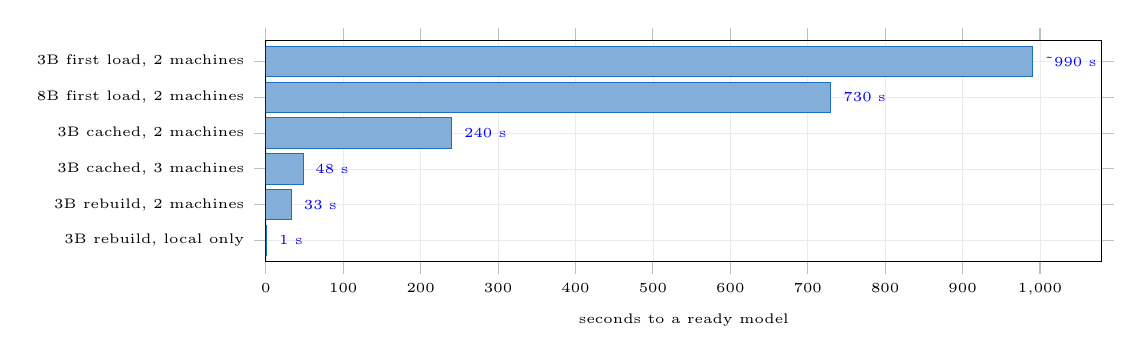
\begin{tikzpicture}[font=\scriptsize]
\begin{axis}[hpaxis,
  width=12.2cm,height=4.4cm,
  xbar, bar width=11pt,
  xmin=0,xmax=1080,
  xlabel={seconds to a ready model},
  symbolic y coords={{3B rebuild, local only},{3B rebuild, 2 machines},{3B cached, 3 machines},{3B cached, 2 machines},{8B first load, 2 machines},{3B first load, 2 machines}},
  ytick=data,
  y tick label style={font=\tiny},
  nodes near coords,
  nodes near coords style={font=\tiny,anchor=west,xshift=1pt},
  enlarge y limits=0.12,
  point meta=explicit symbolic,
  ]
\addplot+[fill=serA!55,draw=serA] coordinates {
  (1,{3B rebuild, local only})      [1 s]
  (33,{3B rebuild, 2 machines})     [33 s]
  (48,{3B cached, 3 machines})      [48 s]
  (240,{3B cached, 2 machines})     [240 s]
  (730,{8B first load, 2 machines}) [730 s]
  (990,{3B first load, 2 machines}) [{\textasciitilde}990 s]
};
\end{axis}
\end{tikzpicture}
\caption{Measured time to a ready model. Each bar is a single observation, not
an average. The two first-load bars include transferring the remote worker's
share of the weights over Wi-Fi on a weak link (\SI{-66}{dBm} to
\SI{-68}{dBm}); once the worker's local tensor cache is populated, the same 3B
model reloads in a small fraction of that time. The cached three-machine load
was measured on the stronger \SI{-56}{dBm} link.}
\label{fig:load}
\end{figure}

The practical consequence is that the first load of a new model on a new worker
is slow and should be done before any demonstration, while subsequent loads and
all recoveries are short. Reported cached 3B loads across sessions were
\SI{240}{\second}, \SI{137}{\second}, \SI{60}{\second} and \SI{48}{\second},
decreasing as link conditions improved; we report the range rather than
selecting the most favourable figure.

\section{Limitations}
\label{sec:limitations}

These are stated plainly because each one changes what the measurements in
Section~\ref{sec:results} mean.

\paragraph{It is slower, not faster.}
Distributing the 3B model over this Wi-Fi network cost roughly a factor of six
in decode throughput against the single local GPU. HyperPod buys aggregate
memory and recovery; it does not buy speed. Anyone whose model already fits on
one machine should run it on one machine.

\paragraph{Recovery restarts, it does not resume.}
When a worker is lost, \texttt{llama.cpp} aborts and HyperPod starts a new
model process and re-runs the request from the beginning. Tokens already
generated are discarded and the KV cache is not preserved. The user sees one
delayed response rather than a partial one, but the work is genuinely repeated.
Continuing from the interrupted token would require state checkpointing inside
the inference engine, which we did not attempt.

\paragraph{The 8B configuration is not fault tolerant on two machines.}
The 8B model does not fit in the controller's \SI{4096}{MiB} GPU alone, so
losing the remote worker leaves nowhere for its \SI{3330}{MiB} share to go.
That configuration demonstrates pooled capacity only. All recovery results in
this report use the 3B model, which the controller can hold by itself.

\paragraph{The scheduler uses memory, not speed.}
Weights are derived from free video memory. Compute throughput, link bandwidth
and link latency are measured and displayed but do not influence placement. A
fast GPU behind a weak link therefore receives the same share as a fast GPU
behind a strong one, which is not optimal.

\paragraph{Metal devices fall back to the engine's own placement.}
Apple Silicon reports no separate free-video-memory figure, so no comparable
weight can be computed for it. Mixed CUDA and Metal clusters use
\texttt{llama.cpp}'s own device probing, reported as
\code{llama.cpp-auto}. The three-machine placement in
Figure~\ref{fig:placement} was chosen by \texttt{llama.cpp}, not by HyperPod.

\paragraph{Joining does not trigger a rebuild.}
A worker that appears after a model is loaded is registered and displayed but is
not added to the running pipeline. Rebuilds happen on failure, not on arrival.
We hit this during our own screenshot session: a freshly started worker sat idle
until the pipeline was rebuilt.

\paragraph{The controller is a single point of failure.}
Worker loss is handled; controller loss is not. If the controller stops, the
cluster stops. Workers do re-register automatically when it returns, but
in-flight work is lost.

\paragraph{No authentication or encryption.}
The \texttt{llama.cpp} RPC backend is documented upstream as insecure, and
HyperPod adds no authentication of its own. The controller API, the worker
endpoints and the discovery broadcast all assume a trusted local network. None
of these ports should be exposed to the internet.

\paragraph{Discovery covers one broadcast domain.}
Workers are found by UDP broadcast, so they must share a subnet with the
controller. Routed networks require explicitly configured endpoints.

\paragraph{The sample sizes are small.}
Performance figures are five runs per configuration on one network on one day.
That is adequate to show a factor-of-six gap between local and distributed
inference, and inadequate to resolve the \SI{0.143}{\second} median difference
between native and HyperPod splits. Each load time in
Figure~\ref{fig:load} is a single observation. Each failure experiment was run
once in the form reported.

\section{Related work}
\label{sec:related}

HyperPod sits on top of existing work rather than replacing it, and the ideas it
uses are not new. This section records what belongs to others.

\paragraph{\texttt{llama.cpp} and its RPC backend.}
All inference here is performed by \texttt{llama.cpp}: GGUF loading,
quantised kernels, CUDA and Metal execution, and the RPC backend that exposes a
remote accelerator. The ability to combine the memory of several machines is
therefore upstream functionality, not ours. What upstream does not provide, and
explicitly describes as out of scope for a proof-of-concept backend, is
surviving the loss of a peer. That gap is what HyperPod addresses.

\paragraph{Consumer-hardware distributed inference.}
Running a single model across several personal devices has been explored by
other projects, including work that schedules layers according to each device's
capability and work that distributes models across volunteer machines over the
public internet. Capability-aware placement in particular is well established;
our scheduler is a deliberately simple instance of it, using one measured
quantity. We make no novelty claim for the idea of weighting devices by
available memory.

\paragraph{Fault tolerance in serving systems.}
Detecting a failed node, excluding it, and restarting work on the survivors is
standard practice in distributed systems and in datacentre model serving. The
mechanisms used here --- heartbeats, health timeouts, endpoint probing, process
supervision, request retry --- are all conventional. Their combination on three
mismatched laptops over domestic Wi-Fi, with the resulting costs measured, is
the part we contribute.

\paragraph{Meta open-weight models.}
The models are Meta's: Llama~3.2 1B and 3B, and Llama~3.1 8B, used as published
GGUF quantisations. HyperPod does not fine-tune or modify them. Access to
open weights is what makes the work possible at all, because the system moves
model weights between physical devices and reads back where they landed. An
API-only model exposes no such surface.

\paragraph{Where this work differs.}
Three things distinguish what is reported here from the surrounding work. The
placement figures are read out of the inference engine's own load output rather
than assumed from the requested split, which is how we found our tensor-order
bug. Unavailable hardware values are preserved as unavailable all the way to the
interface, so the Mac's missing video-memory figure is visible instead of being
filled in. And the failure experiments were performed by stopping real processes
on real machines during live requests, with the resulting logs committed, rather
than by injecting faults in software.

\section{Conclusion}

HyperPod turns three mismatched consumer laptops into a single local runtime for
Meta open-weight models, and keeps serving when one of them stops.

The measurements in this report establish four things on real hardware. A
Llama~3.2~3B model was placed across a Linux RTX~3050, a Windows RTX~4050 and an
M4 MacBook~Air, with the per-device byte counts read back from
\texttt{llama.cpp} rather than assumed. Stopping the Mac accelerator mid-request
caused the inference process to abort, after which HyperPod excluded the
unreachable endpoint, rebuilt a still-distributed pipeline across the two
survivors in \SI{33}{\second}, and returned the same HTTP request without
resubmission; under the same conditions unmodified \texttt{llama.cpp} failed the
request and did not restart. A Llama~3.1~8B model that does not fit in the
controller's \SI{4096}{MiB} GPU ran with \SI{3330}{MiB} of its weights on the
remote Windows GPU. And distributing over Wi-Fi cost roughly a factor of six in
decode throughput relative to the single local GPU.

The last of those is as important as the first three. This design trades
throughput for capacity and for recovery. On a network like ours the trade only
makes sense when the model does not fit on one machine, or when an interrupted
request matters more than its latency.

What we would build next follows from Section~\ref{sec:limitations}. Caching
model weights on each worker's disk ahead of time would remove the long first
load, which is currently the worst part of the experience. Adding measured
compute and link bandwidth to the scheduler would let it place work on the
machine that can actually do it fastest, rather than the one with the most free
memory. Preserving the KV cache across a rebuild would turn restart-and-retry
into genuine continuation. Controller election would remove the last single
point of failure. Authentication would make the system safe outside a trusted
network.

Every figure quoted here is reproducible from the committed logs under
\code{test/} in the repository, and the two physical failure experiments are
recorded in \code{test/phase6-three-node-recovery.log} and
\code{test/phase7-native-benchmark.log}.

\vspace{1em}
\noindent\textbf{Built with Llama.} Llama 3.1 and Llama 3.2 are licensed by Meta
under their respective Community License Agreements. \texttt{llama.cpp} is used
under the MIT License. Full notices are in \code{THIRD\_PARTY\_NOTICES.md}.


\end{document}
